\documentclass[11pt]{article}

\title{Teknologipr  osjekt: Øving 2}
\author{Mathias Mellemstuen, Tobias Hallingstad, Ruben Fosby, Henrik Bratseth, Andreas Thauland, Erik Holmen}
\date{16.10.20}
\pdfoutput=1

\usepackage{changepage}
\usepackage[margin=1in]{geometry}
\usepackage[dvipsnames]{color}
\usepackage{url}
\usepackage{pgfgantt}
\usepackage{graphicx}

\newenvironment{myenv}{\begin{adjustwidth}{1cm}{}}{\end{adjustwidth}}

\begin{document}
\begin{center}
\section*{Teknologiprosjekt: Øving 2}
\textbf{Planning report}
\line(1,0){400}
\end{center}
The project fits for industrial warehouses, hospitals and anywhere robots are suited to move things around automatically. There is a lack of cheap options in the current state of the art.
\\Our expected outcome is to make a robot follow a painted line, using a camera and detect objects in its path using an ultrasonic range finder. The robot should be able to move on any track and make decisions in real time.
The overall goal is to create a cost-efficient line-following robot that can do simple tasks such as carrying cargo from A to B. The robot should be able work in different scenarios (harbor, warehouse, hospitals etc).
\\\\
\textbf{Requirements}\\
There are a few requirements and tasks that we will follow in order to get this robot to do what we want, here is a specified list over some of them:
\begin{itemize}
    \item Following any track with specific requirements. We were instructed to make our robot do the following: \begin{itemize}
        \item Keep itself on the right hand lane, as if it was a car on a real road.
        \item Turn right on every intersection or turn. (We are planning on implementing the ability to do more than just turning right, but we will keep this as the default as that is what we were instructed to do.)
    \end{itemize} 
    \item Regulate angular and linear velocity. \begin{itemize}
        \item It is important for the robot to be able to adjust its velocity in order to not overshoot turns.
    \end{itemize}
    \item Detect obstacles and respond to them. \begin{itemize}
        \item Configuring the visual sensor to detect obstacles within a certain range and slowing down to a halt in order to not crash into anything. 
    \end{itemize}
    \item Carry small items as cargo. \begin{itemize}
        \item The robot has a flat surface with a few screws sticking up, which are ideal to carry smaller objects.
    \end{itemize}
    \item Control and get values / status in a web interface. \begin{itemize}
        \item We will use a website as an interface, and implement remote controls to be able to take over and “drive” our robot. This interface will also contain values such as speed, angles and a live feed of what the robot is seeing through the cameras. 
    \end{itemize}
\end{itemize}
\textbf{Limitations}
\\
As with any project there are limitations, either things we don’t have the ability to do or lack of time and resources. Here are a few we stumbled across: 
\begin{itemize}
	\item Obstacle detection. \begin{itemize}
        \item We are unable to make the robot move around obstacles, it can only stop and wait for the object to be removed.
    \end{itemize}
	\item Cargo weight. \begin{itemize}
        \item The cargo can’t be too heavy as the robot lacks the power to carry heavier items.
        \item The robot also lacks the ability to adjust speed according to the weight of the items carried, so the robot might lose cargo by going too fast.
    \end{itemize}
	\item Line detection. \begin{itemize}
        \item The track can only be made of a single colour for contrast comparison.
    \end{itemize}
\end{itemize}
\textbf{Motion control algorithm}
\\
In order to make the robot do its job, we need a motion control algorithm that at least loosely follows the points under:
\begin{enumerate}
    \item Sample input data from the distance sensor and stop the robot if the distance is within a certain value. \begin{itemize}
        \item We will install a distance sensor on the front end of the robot, we will then be able to measure how far the robot currently is from an object that is in its path. The robot will then be able to stop when he is within x mm of the object. 
    \end{itemize}
    \item Check data from the image processing if the track exists in the image. \begin{itemize}
        \item On track: Goto point 3. 
        \item Not on track: Drive around in circles until the track is found.
    \end{itemize}
    \item Check if the robot is near a crossroad. \begin{itemize}
        \item On crossroad: Move either left. right or forward. The robot can be hardcoded to always move in one direction or take a random direction. 
        \item Not on crossroad: Go to point 4. 
    \end{itemize}
    \item Find the shortest distance and angle to the middle of the track. This will be the general direction / the next destination. 
    \item Calculate angular and linear velocity according to the data sampled in point 3. 
    \item Check if it has reached it's final destination or goal. If that is not the case, go to point 1.
\end{enumerate}
\textbf{I/O module}
\\
This module contains code for every sensor on the robot, including output to the motors. This module will be responsible for connecting every other module together, it will be the core code of the robot. 
\\\\
\begin{myenv}

    \textbf{Camera module}
    \\
    The project includes a Raspberry Pi camera. We will use the standard raspberry Pi camera library to receive images from the camera. Then we will use OpenCV to convert the image to an array of pixels.
    \\\\
    \textbf{Distance sensor}
    \\ 
    The project includes a distance sensor. The GoPiGo library contains a function that returns the distance to the obstacles in millimetres which we can use further in the code. 
    \\\\
    \textbf{Motor I/O}
    \\
    A function to control the wheels of the robot. The function should take two parameters, one for the speed of the wheel and another that defines which wheel to set the speed. \\
\end{myenv}
\textbf{Image processing module}
\\
In order for the robot to detect the road it’s going to follow it will have to process images in real time, these images will be converted and scanned in order to make this as easy as possible:
\begin{itemize}
    \item Get the image as an array of pixels from the I/O module. 
    \item Convert the colors in the array to black/white. \begin{itemize}
        \item The robot is very limited when it comes to detecting colours, so to overcome that hurdle we will grayscale the image and use contrasting to make the image into black and white in order to detect the opposing colours.
    \end{itemize}
    \item Use the Hough transform algorithm to find the edges of the track. \begin{itemize}
        \item Using the Hough transform algorithm we can find the edges of the track, with these we can create a sort of coordination system that will tell the robot where to go.
    \end{itemize}
    \item Find the middle of the road. \begin{itemize}
        \item When we have the edges of the track and the coordination system it is easy to find the middle of the lane and stick to it.
    \end{itemize}
    \item Return the middle of the road and the robots offset to the middle. 
\end{itemize}
\textbf{User interface} 
\\
The user interface is a web page that is locally hosted on the raspberry pi. The webserver is running within the python program. The web page is using API calls to collect data / give command to the python program. All of this is happening asynchronous with the rest of the python code. 
\\\\
\textbf{Installation and deployment of the solution (Implementation)}
In order to implement and deploy our solution we will follow these steps:
\begin{enumerate}
    \item Installing the raspbian OS on a microSD card. 
    \item Setting up the raspberry pi to host a WIFI network. 
    \item Creating users for each group member on the linux system.
    \item Setting up SSH. 
    \item Installing the GoPiGo libraries from github. 
    \item Opening port 80 on the firewall for the web interface. 
    \item Setting up a service in systemctl to run the python code when linux is booting.
\end{enumerate}
Here is a visual representation of how all the different modules connects: 
\begin{center}
    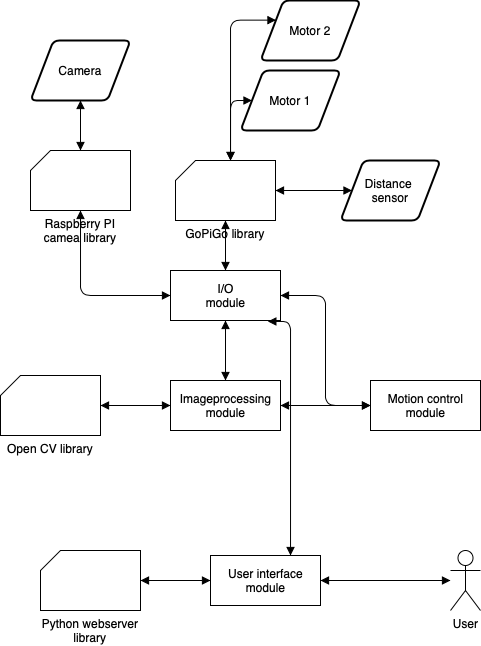
\includegraphics[width=0.5\textwidth]{flowdiagram}
\end{center}
\textbf{Responsibilities} \\
This is a list of the different responsibilities of the work packages. Everyone will do work in the different work packages, this list is only showing who is in charge of managing and leading the current work package. \\\\
\begin{tabular}{ |c|c| }
    \hline
    \textbf{Work package (WP)} & \textbf{Responsibility} \\
    \hline
    I/O module & Mathias \\
    \hline
    Motion control module & Tobias \\
    \hline
    Image processing module & Henrik \\
    \hline
    Web interface & Ruben \\
    \hline
    Testing & Andreas \\
    \hline
    Documentation & Erik \\
    \hline
\end{tabular}
\\\\\\
\textbf{Gantt chart}
\\
This Gantt chart is visualizing the planned workflow of the project. 
\begin{center}
    \begin{ganttchart}[%Specs
             y unit title=0.5cm,
             y unit chart=0.7cm,
             vgrid,hgrid,
             title height=1,
             %     title/.style={fill=none},
             title label font=\bfseries\footnotesize,
                  bar/.style={fill=blue},
                  bar height=0.7,
                  %   progress label text={},
                  group right shift=0,
                  group top shift=0.7,
                  group height=.3,
                  group peaks width={0.2},
                  inline]{1}{15}
              %labels
              %    \gantttitle{A project}{15}\\  % title level 1
              \gantttitle[]{Aug.}{2}             % title level 2
              \gantttitle[]{September}{4}                
              \gantttitle[]{October}{5}               
              \gantttitle[]{November}{4} \\      
    
              % I/O Module
              \ganttgroup[inline=false]{WP 1: I/O Module}{1}{7} \\ 
              \ganttbar[inline=false]{General setup}{1}{2} \\
              \ganttmilestone[inline=false]{Milestone: Setup}{2} \\
              \ganttbar[inline=false]{Camera}{3}{5} \\
              \ganttmilestone[inline=false]{Milestone: Camera}{5} \\
              \ganttbar[inline=false]{Distance sensor}{6}{7} \\
              \ganttmilestone[inline=false]{Milestone: R3}{7} \\
              
              % Motion control
              \ganttgroup[inline=false]{WP 2: Motion control}{1}{13} \\
              \ganttbar[inline=false]{Driving}{1}{2} \\
              \ganttbar[inline=false]{Turning}{3}{4} \\
              \ganttbar[inline=false]{Motion control algorithm}{5}{7} \\
              \ganttmilestone[inline=false]{Milestone: Simple control}{7} \\
              \ganttbar[inline=false]{Stoping}{8}{9} \\
              \ganttbar[inline=false]{Cross lane turning}{10}{11} \\
              \ganttmilestone[inline=false]{Milestone: done}{11} \\
              \ganttbar[inline=false]{Testing}{12}{13} \\
              
              % Image processing
              \ganttgroup[inline=false]{WP 3: Image processing}{1}{12} \\ 
              \ganttbar[inline=false]{Lane detection}{1}{3} \\ 
              \ganttbar[inline=false]{Single straight lane}{4}{5} \\ 
              \ganttmilestone[inline=false]{Milestone 1}{5} \\       
              \ganttbar[inline=false]{Single curved lane}{6}{7} \\ 
              \ganttbar[inline=false]{Cross lane detection}{8}{10} \\ 
              \ganttmilestone[inline=false]{Milestone Cross lane}{10} \\
              \ganttbar[inline=false]{Testing}{11}{12} \\
    
              % Web interface
              \ganttgroup[inline=false]{WP 4: Web interface}{3}{10} \\
              \ganttbar[inline=false]{Web design}{3}{10} \\
              \ganttbar[inline=false]{Display info}{3}{4} \\
              \ganttbar[inline=false]{Variable control}{4}{5} \\
              \ganttmilestone[inline=false]{Milestone: general variable change}{5} \\
              \ganttbar[inline=false]{Display camera}{6}{7} \\
              \ganttmilestone[inline=false]{Milestone: Camera streaming}{7} \\
              \ganttbar[inline=false]{Camera filter}{8}{9} \\
              \ganttmilestone[inline=false]{Milestone: Display camera filters}{9} \\
              \ganttbar[inline=false]{Robot control}{8}{10} \\
              \ganttmilestone[inline=false]{Milestone: Controlling robot}{10}
    
         \end{ganttchart}
    \end{center}
    
    \begin{center}
         \begin{ganttchart}[%Specs
              y unit title=0.5cm,
              y unit chart=0.7cm,
              vgrid,hgrid,
              title height=1,
              %     title/.style={fill=none},
              title label font=\bfseries\footnotesize,
                   bar/.style={fill=blue},
                   bar height=0.7,
                   %   progress label text={},
                   group right shift=0,
                   group top shift=0.7,
                   group height=.3,
                   group peaks width={0.2},
                   inline]{1}{15}
              %labels
              %    \gantttitle{A project}{15}\\  % title level 1
              \gantttitle[]{Aug.}{2}             % title level 2
              \gantttitle[]{September}{4}                
              \gantttitle[]{October}{5}               
              \gantttitle[]{November}{4} \\ 
    
              % Testing
              \ganttgroup[inline=false]{WP 5: Testing}{2}{15} \\
              \ganttbar[inline=false]{WP 1 testing}{2}{7} \\
              \ganttbar[inline=false]{WP 2 testing}{8}{12} \\
              \ganttbar[inline=false]{WP 3 testing}{6}{11} \\
              \ganttbar[inline=false]{WP 4 testing}{6}{10} \\
              \ganttmilestone[inline=false]{Milestone: Done testing}{12} \\
              \ganttbar[inline=false]{Final testing}{13}{15} \\
              \ganttmilestone[inline=false]{Project done}{15} \\
    
              % Documentation
              \ganttgroup[inline=false]{WP 6: Documentation}{1}{15} \\ \\
    
              %% Doc WP 1 I/O
              \ganttgroup[inline=false]{WP 6.1: I/O Module doc}{2}{8} \\
              \ganttbar[inline=false]{WP 1: General}{2}{3} \\
              \ganttbar[inline=false]{WP 1: Camera}{5}{6} \\
              \ganttbar[inline=false]{WP 1: Distance sensor}{7}{8} \\
              \ganttmilestone[inline=false]{Wp 1: Doc done}{8} \\
    
              %% Doc WP 2 Motion control
              \ganttgroup[inline=false]{WP 6.2: Motion controll doc}{3}{12} \\
              \ganttbar[inline=false]{WP 2: Driving}{3}{4} \\
              \ganttbar[inline=false]{WP 2: Turning}{4}{5} \\
              \ganttbar[inline=false]{WP 2: Motion control algorithm}{6}{8} \\
              \ganttbar[inline=false]{WP 2: Stopping}{9}{10} \\
              \ganttbar[inline=false]{WP 2: Cross lane}{11}{12} \\
              \ganttmilestone[inline=false]{WP 2: Doc done}{12} \\
    
              %% Doc WP 3 Image prossesing
              \ganttgroup[inline=false]{WP 6.3: Image processing doc}{3}{10} \\
              \ganttbar[inline=false]{WP 3: Lane detection}{3}{4} \\
              \ganttbar[inline=false]{WP 3: Singel straight lane}{5}{6} \\
              \ganttbar[inline=false]{WP 3: Single curved lane}{7}{8} \\
              \ganttbar[inline=false]{WP 3: Cross lane detection}{9}{10} \\
              \ganttmilestone[inline=false]{WP 3: Doc done}{10} \\
    
              %% Doc WP 4 Web interface
              \ganttgroup[inline=false]{WP 6.4: Web interface doc}{10}{12} \\
              \ganttbar[inline=false]{WP 4: Display Info}{10}{10} \\
              \ganttbar[inline=false]{WP 4: Variable control}{10}{10} \\
              \ganttbar[inline=false]{WP 4: Display Camera}{11}{11} \\
              \ganttbar[inline=false]{WP 4: Display Camera filter}{11}{11} \\
              \ganttbar[inline=false]{WP 4: Display Control robot}{12}{12} \\
              \ganttmilestone[inline=false]{WP 4: Doc done}{12}
    
         \end{ganttchart}
    \end{center}
\textbf{Risks}\\
There are always risks when implementing projects like this, some of the risks we can experience are: 
\begin{itemize}
    \item Camera lacking the resolution for our image processing algorithm. \begin{itemize}
        \item One of the problems we might face is that the camera we are using will not work with our image processing algorithm. Some of the reasons it might not work is resolution or other specifications limitations on the camera we are using. 
    \end{itemize}
    \item Defect components (camera, distance sensor, etc.) \begin{itemize}
        \item A risk when making a project that has multiple components is of course that some of the components we are using are broken in some way, this can be either easy to see physical damage and it can be hard to find internal damage. 
    \end{itemize}
    \item Bad placement of critical components (camera, distance sensor, etc.) \begin{itemize}
        \item if the camera angle is either too high or too low the image processing could give bad results.
    \end{itemize}
    \item Code that doesn’t work the way we intended. \begin{itemize}
        \item This could include everything from bugs and bad implementation to too high/low values.
    \end{itemize}
    \item Bad time management. \begin{itemize}
        \item When working on a larger project we run the risk of giving each task too much or too little time. 
    \end{itemize}
\end{itemize}
\textbf{Mitigation}\\
Some of the ways we can hopefully mitigate these risks are:
\begin{itemize}
    \item Make sure that the components we use all have good enough specifications while still being affordable. \begin{itemize}
        \item We can reduce the risk of limitations from components by carefully planning which components we need to use, finding out what specifications these components need to have, and making sure that we atleast fulfill the minimum requirements. 
    \end{itemize}
    \item Make sure that all components are working by thoroughly testing them before deployment. \begin{itemize}
        \item This includes doing a physical inspection of them to try to see any broken parts, as well as thoroughly testing them before deployment. 
    \end{itemize}
    \item Thoroughly testing the code at each stage, to catch errors early and squash bugs. 
    \item We can hopefully mitigate bad time management by thoroughly discussing and planning the project.  
\end{itemize}
\end{document}  